\documentclass{standalone}
\usepackage{tikz}
\usetikzlibrary{patterns, positioning}

\begin{document}
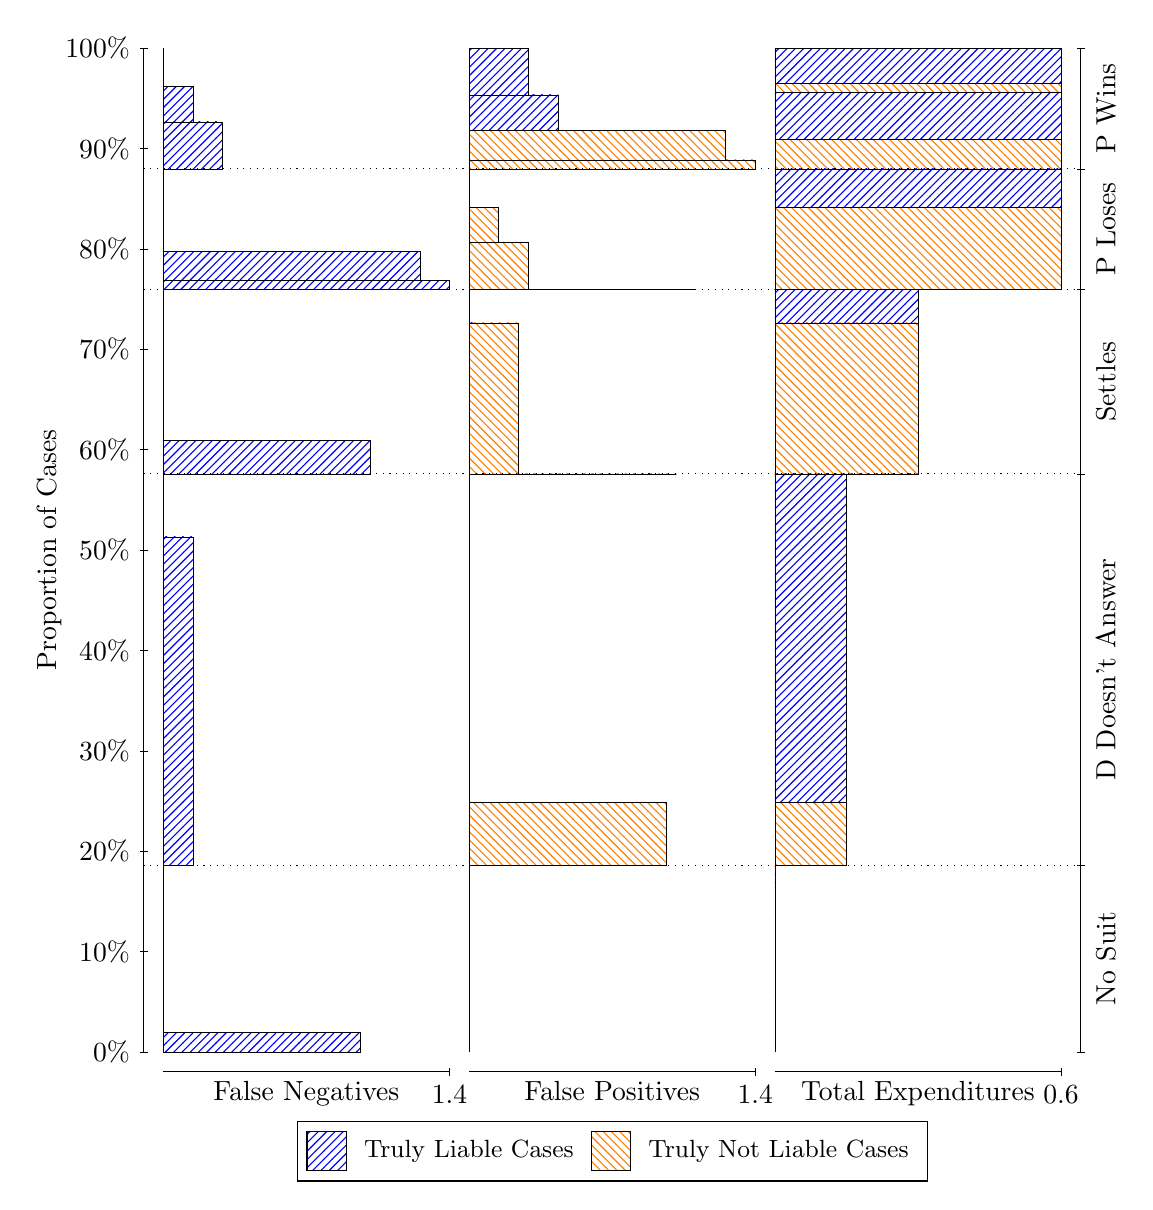
\begin{tikzpicture}
\draw[black, very thin] (1.5,1.75) -- (1.5,14.5);
\node[rotate=90, anchor=center] at (0.3, 8.125) {Proportion of Cases};
\draw[black, very thin] (1.45,1.75) -- (1.55,1.75);
\node[anchor=east] at (1.45, 1.75) {0\%};
\draw[black, very thin] (1.45,3.025) -- (1.55,3.025);
\node[anchor=east] at (1.45, 3.025) {10\%};
\draw[black, very thin] (1.45,4.3) -- (1.55,4.3);
\node[anchor=east] at (1.45, 4.3) {20\%};
\draw[black, very thin] (1.45,5.575) -- (1.55,5.575);
\node[anchor=east] at (1.45, 5.575) {30\%};
\draw[black, very thin] (1.45,6.85) -- (1.55,6.85);
\node[anchor=east] at (1.45, 6.85) {40\%};
\draw[black, very thin] (1.45,8.125) -- (1.55,8.125);
\node[anchor=east] at (1.45, 8.125) {50\%};
\draw[black, very thin] (1.45,9.4) -- (1.55,9.4);
\node[anchor=east] at (1.45, 9.4) {60\%};
\draw[black, very thin] (1.45,10.675) -- (1.55,10.675);
\node[anchor=east] at (1.45, 10.675) {70\%};
\draw[black, very thin] (1.45,11.95) -- (1.55,11.95);
\node[anchor=east] at (1.45, 11.95) {80\%};
\draw[black, very thin] (1.45,13.225) -- (1.55,13.225);
\node[anchor=east] at (1.45, 13.225) {90\%};
\draw[black, very thin] (1.45,14.5) -- (1.55,14.5);
\node[anchor=east] at (1.45, 14.5) {100\%};

\draw[black, very thin] (13.4,1.75) -- (13.4,14.5);
\draw[black, very thin] (13.35,1.75) -- (13.45,1.75);
\node[anchor=west] at (13.35, 1.75) {};
\draw[black, very thin] (13.35,4.1224) -- (13.45,4.1224);
\node[anchor=west] at (13.35, 4.1224) {};
\draw[black, very thin] (13.35,9.0921) -- (13.45,9.0921);
\node[anchor=west] at (13.35, 9.0921) {};
\draw[black, very thin] (13.35,11.432) -- (13.45,11.432);
\node[anchor=west] at (13.35, 11.432) {};
\draw[black, very thin] (13.35,11.432) -- (13.45,11.432);
\node[anchor=west] at (13.35, 11.432) {};
\draw[black, very thin] (13.35,12.966) -- (13.45,12.966);
\node[anchor=west] at (13.35, 12.966) {};
\draw[black, very thin] (13.35,14.5) -- (13.45,14.5);
\node[anchor=west] at (13.35, 14.5) {};

\draw[black, very thin, pattern color=blue, pattern=north east lines] (1.75,1.75) rectangle (4.2557,1.9996);
\draw[black, very thin, pattern color=orange, pattern=north west lines] (1.75,1.9996) rectangle (1.75,4.1224);
\draw[black, very thin, pattern color=blue, pattern=north east lines] (1.75,4.1224) rectangle (2.1259,8.2905);
\draw[black, very thin, pattern color=orange, pattern=north west lines] (1.75,8.2905) rectangle (1.75,9.0921);
\draw[black, very thin, pattern color=blue, pattern=north east lines] (1.75,9.0921) rectangle (4.381,9.5154);
\draw[black, very thin, pattern color=blue, pattern=north east lines] (1.75,9.5154) rectangle (4.1305,9.5154);
\draw[black, very thin, pattern color=blue, pattern=north east lines] (1.75,9.5154) rectangle (3.8799,9.5154);
\draw[black, very thin, pattern color=blue, pattern=north east lines] (1.75,9.5154) rectangle (3.6293,9.5154);
\draw[black, very thin, pattern color=blue, pattern=north east lines] (1.75,9.5154) rectangle (3.3787,9.5154);
\draw[black, very thin, pattern color=blue, pattern=north east lines] (1.75,9.5154) rectangle (3.1282,9.5154);
\draw[black, very thin, pattern color=blue, pattern=north east lines] (1.75,9.5154) rectangle (2.8776,9.5154);
\draw[black, very thin, pattern color=blue, pattern=north east lines] (1.75,9.5154) rectangle (2.627,9.5154);
\draw[black, very thin, pattern color=blue, pattern=north east lines] (1.75,9.5154) rectangle (2.3764,9.5154);
\draw[black, very thin, pattern color=orange, pattern=north west lines] (1.75,9.5154) rectangle (1.75,11.432);
\draw[black, very thin, pattern color=blue, pattern=north east lines] (1.75,11.432) rectangle (2.1259,11.432);
\draw[black, very thin, pattern color=orange, pattern=north west lines] (1.75,11.432) rectangle (1.75,11.432);
\draw[black, very thin, pattern color=blue, pattern=north east lines] (1.75,11.432) rectangle (5.3833,11.545);
\draw[black, very thin, pattern color=blue, pattern=north east lines] (1.75,11.545) rectangle (5.0075,11.918);
\draw[black, very thin, pattern color=orange, pattern=north west lines] (1.75,11.918) rectangle (1.75,12.966);
\draw[black, very thin, pattern color=blue, pattern=north east lines] (1.75,12.966) rectangle (2.5017,13.561);
\draw[black, very thin, pattern color=blue, pattern=north east lines] (1.75,13.561) rectangle (2.1259,14.014);
\draw[black, very thin, pattern color=orange, pattern=north west lines] (1.75,14.014) rectangle (1.75,14.5);
\draw[black, very thin, pattern color=orange, pattern=north west lines] (5.6333,1.75) rectangle (5.6333,3.8728);
\draw[black, very thin, pattern color=blue, pattern=north east lines] (5.6333,3.8728) rectangle (5.6333,4.1224);
\draw[black, very thin, pattern color=orange, pattern=north west lines] (5.6333,4.1224) rectangle (8.1391,4.924);
\draw[black, very thin, pattern color=blue, pattern=north east lines] (5.6333,4.924) rectangle (5.6333,9.0921);
\draw[black, very thin, pattern color=orange, pattern=north west lines] (5.6333,9.0921) rectangle (8.2644,9.0921);
\draw[black, very thin, pattern color=orange, pattern=north west lines] (5.6333,9.0921) rectangle (8.0138,9.0921);
\draw[black, very thin, pattern color=orange, pattern=north west lines] (5.6333,9.0921) rectangle (7.7632,9.0921);
\draw[black, very thin, pattern color=orange, pattern=north west lines] (5.6333,9.0921) rectangle (7.5126,9.0921);
\draw[black, very thin, pattern color=orange, pattern=north west lines] (5.6333,9.0921) rectangle (7.2621,9.0921);
\draw[black, very thin, pattern color=orange, pattern=north west lines] (5.6333,9.0921) rectangle (7.0115,9.0921);
\draw[black, very thin, pattern color=orange, pattern=north west lines] (5.6333,9.0921) rectangle (7.0115,9.0921);
\draw[black, very thin, pattern color=orange, pattern=north west lines] (5.6333,9.0921) rectangle (6.7609,9.0921);
\draw[black, very thin, pattern color=orange, pattern=north west lines] (5.6333,9.0921) rectangle (6.5103,9.0921);
\draw[black, very thin, pattern color=orange, pattern=north west lines] (5.6333,9.0921) rectangle (6.2598,11.009);
\draw[black, very thin, pattern color=blue, pattern=north east lines] (5.6333,11.009) rectangle (5.7586,11.009);
\draw[black, very thin, pattern color=blue, pattern=north east lines] (5.6333,11.009) rectangle (5.6333,11.432);
\draw[black, very thin, pattern color=orange, pattern=north west lines] (5.6333,11.432) rectangle (8.5149,11.432);
\draw[black, very thin, pattern color=blue, pattern=north east lines] (5.6333,11.432) rectangle (6.0092,11.432);
\draw[black, very thin, pattern color=orange, pattern=north west lines] (5.6333,11.432) rectangle (6.3851,12.027);
\draw[black, very thin, pattern color=orange, pattern=north west lines] (5.6333,12.027) rectangle (6.0092,12.48);
\draw[black, very thin, pattern color=blue, pattern=north east lines] (5.6333,12.48) rectangle (5.6333,12.966);
\draw[black, very thin, pattern color=orange, pattern=north west lines] (5.6333,12.966) rectangle (9.2667,13.079);
\draw[black, very thin, pattern color=orange, pattern=north west lines] (5.6333,13.079) rectangle (8.8908,13.452);
\draw[black, very thin, pattern color=blue, pattern=north east lines] (5.6333,13.452) rectangle (6.7609,13.905);
\draw[black, very thin, pattern color=blue, pattern=north east lines] (5.6333,13.905) rectangle (6.3851,14.5);
\draw[black, very thin, pattern color=orange, pattern=north west lines] (9.5167,1.75) rectangle (9.5167,3.8728);
\draw[black, very thin, pattern color=blue, pattern=north east lines] (9.5167,3.8728) rectangle (9.5167,4.1224);
\draw[black, very thin, pattern color=orange, pattern=north west lines] (9.5167,4.1224) rectangle (10.425,4.924);
\draw[black, very thin, pattern color=blue, pattern=north east lines] (9.5167,4.924) rectangle (10.425,9.0921);
\draw[black, very thin, pattern color=orange, pattern=north west lines] (9.5167,9.0921) rectangle (11.333,9.0921);
\draw[black, very thin, pattern color=blue, pattern=north east lines] (9.5167,9.0921) rectangle (11.333,9.0921);
\draw[black, very thin, pattern color=orange, pattern=north west lines] (9.5167,9.0921) rectangle (11.333,11.009);
\draw[black, very thin, pattern color=blue, pattern=north east lines] (9.5167,11.009) rectangle (11.333,11.432);
\draw[black, very thin, pattern color=orange, pattern=north west lines] (9.5167,11.432) rectangle (11.333,11.432);
\draw[black, very thin, pattern color=blue, pattern=north east lines] (9.5167,11.432) rectangle (11.333,11.432);
\draw[black, very thin, pattern color=orange, pattern=north west lines] (9.5167,11.432) rectangle (11.333,11.432);
\draw[black, very thin, pattern color=blue, pattern=north east lines] (9.5167,11.432) rectangle (11.333,11.432);
\draw[black, very thin, pattern color=orange, pattern=north west lines] (9.5167,11.432) rectangle (13.15,12.48);
\draw[black, very thin, pattern color=blue, pattern=north east lines] (9.5167,12.48) rectangle (13.15,12.966);
\draw[black, very thin, pattern color=orange, pattern=north west lines] (9.5167,12.966) rectangle (13.15,13.339);
\draw[black, very thin, pattern color=blue, pattern=north east lines] (9.5167,13.339) rectangle (13.15,13.934);
\draw[black, very thin, pattern color=orange, pattern=north west lines] (9.5167,13.934) rectangle (13.15,14.047);
\draw[black, very thin, pattern color=blue, pattern=north east lines] (9.5167,14.047) rectangle (13.15,14.5);
\draw[black, dotted] (1.5,4.1224) -- (13.4,4.1224);
\draw[black, dotted] (1.5,9.0921) -- (13.4,9.0921);
\draw[black, dotted] (1.5,11.432) -- (13.4,11.432);
\draw[black, dotted] (1.5,11.432) -- (13.4,11.432);
\draw[black, dotted] (1.5,12.966) -- (13.4,12.966);
\draw[black, very thin] (1.75,1.5) -- (5.3833,1.5);
\node[anchor=north] at (3.5667, 1.5) {False Negatives};
\draw[black, very thin] (5.3833,1.45) -- (5.3833,1.55);
\node[anchor=north] at (5.3833, 1.45) {1.4};

\draw[black, very thin] (5.6333,1.5) -- (9.2667,1.5);
\node[anchor=north] at (7.45, 1.5) {False Positives};
\draw[black, very thin] (9.2667,1.45) -- (9.2667,1.55);
\node[anchor=north] at (9.2667, 1.45) {1.4};

\draw[black, very thin] (9.5167,1.5) -- (13.15,1.5);
\node[anchor=north] at (11.333, 1.5) {Total Expenditures};
\draw[black, very thin] (13.15,1.45) -- (13.15,1.55);
\node[anchor=north] at (13.15, 1.45) {0.6};

\node[black, centered, rotate=90] at (13.72, 2.9362) {No Suit};
\node[black, centered, rotate=90] at (13.72, 6.6072) {D Doesn't Answer};
\node[black, centered, rotate=90] at (13.72, 10.262) {Settles};

\node[black, centered, rotate=90] at (13.72, 12.199) {P Loses};
\node[black, centered, rotate=90] at (13.72, 13.733) {P Wins};

\draw (7.449999999999999,1.5) node[draw=none] (baseCoordinate) {};
\begin{scope}[align=center]
        \matrix[scale=0.5, draw=black, below=0.5cm of baseCoordinate, nodes={draw}, column sep=0.1cm]{
            \node[rectangle, draw, minimum width=0.5cm, minimum height=0.5cm, pattern=north east lines, pattern color=blue] {}; &
            \node[draw=none, font=\small] (B) {Truly Liable Cases}; &
            \node[rectangle, draw, minimum width=0.5cm, minimum height=0.5cm, pattern=north west lines, pattern color=orange] {}; &
            \node[draw=none, font=\small] (B) {Truly Not Liable Cases}; \\
            };
\end{scope}

\end{tikzpicture}
\end{document}